\chapter{Základní pojmy}

\section{Šum}

V teorii detekce signálu šumem nazýváme jakoukoli nechtěnou (a typicky neznámou) modifikaci signálu.

\subsection{Barva šumu}

U aditivního\footnote{Šumu říkáme aditivní, pokud se jeho hodnoty přičítají k
hodnotě signálu. Dále existuje například ještě šum multiplikativní či fázový
(šum, který se projevuje krátkodobým fázovám posunem signálu).} šumu můžeme
měřit intenzitu šumu na různých frekvencích. Tu změříme tak, že na šum aplikujeme
Fourierovu transformaci

 Šumu se
říká bílý šum, pokud by světlo, které by mělo stejnou distribuci intenzity
napříč frekvencemi, jako daný šum (který ale vůbec nemusí být světelný), bylo
bílé. Podobně známe například ještě růžový, červený či modrý šum.

Intenzita $p$ všech zmíněných šumů na v na dané frekvenci lze vyjádřit jako
$p=1/f^\beta$, kde hodnota $\beta$ je $-1$ pro modrý šum, $0$ pro bílý, $1$ pro
růžový a $2$ pro hnědý. Proto se růžový šum někdy též označuje jako $1/f$ šum. Pro
ostatní barvy šumu není podobné označení běžné.

Pravděpodobnostní rozdělení jednotlivých složek Fourierovy transformace ale
není definicí barvy šumu dáno. Pokud je rozdělení normální\footnote{Nezáleží na
tom, zda má normální rozdělení šum sám nebo jeho Fourierův obraz -- tyto dvě
vlastnosti jsou ekvivalentní.}, řekneme, že se jedná o Gaussovský šum. 

V této práci se budeme zabývat vizuálním šumem, tedy šumem, kde místo obvykle
používané časové souřadnice použijeme dvě souřadnice prostorové, a měřenou
hodnotou bude jas. 

\begin{figure}[h!]
\begin{tabular}{cc}
\begin{subfigure}{0.45\textwidth}
  \centering
  
\includegraphics[width=.8\linewidth]{img/blue_noise}
  \caption{Modrý šum} 
\end{subfigure}&
\begin{subfigure}{0.45\textwidth}
  \centering
  
\includegraphics[width=.8\linewidth]{img/white_noise}
  \caption{Bílý šum} 
\end{subfigure}\\
\begin{subfigure}{0.45\textwidth}
  \centering
  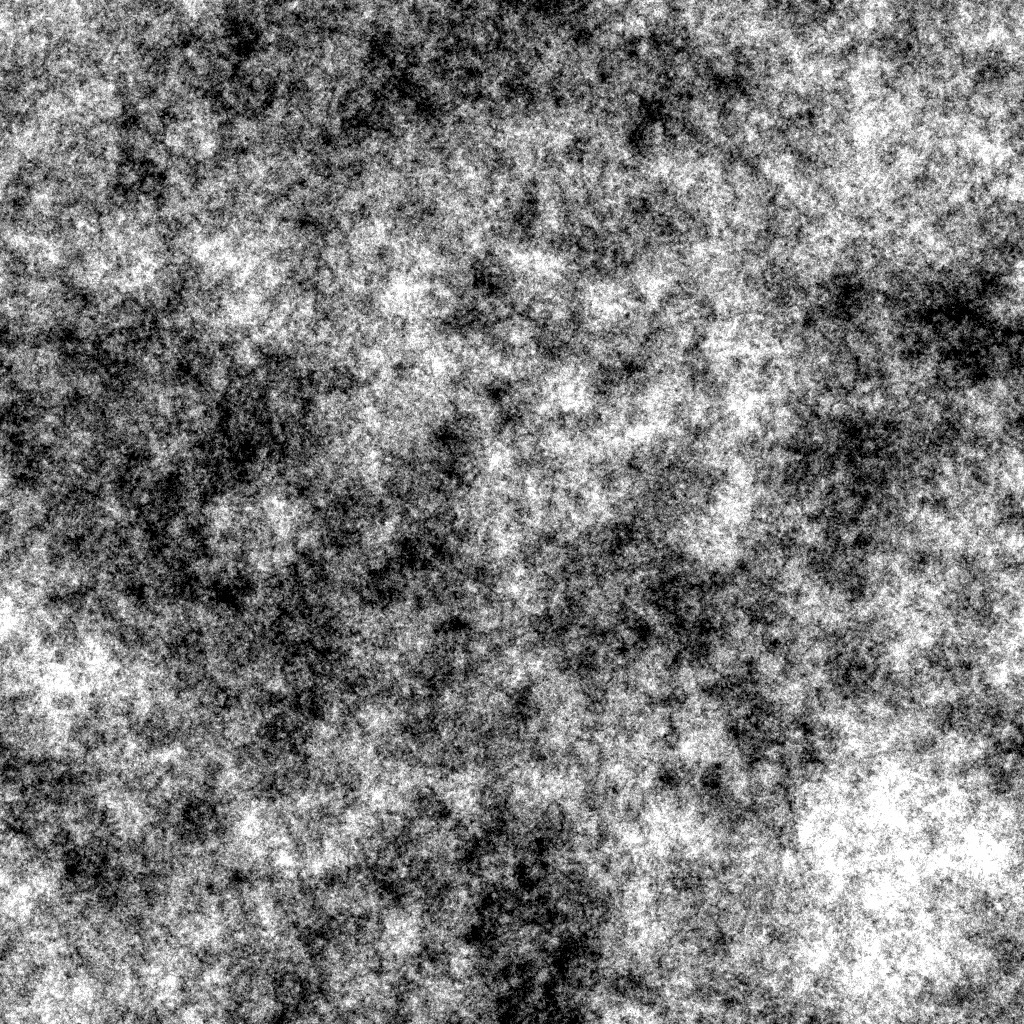
\includegraphics[width=.8\linewidth]{img/pink_noise}
  \caption{Růžový šum} 
\end{subfigure}&
\begin{subfigure}{0.45\textwidth}
  \centering
  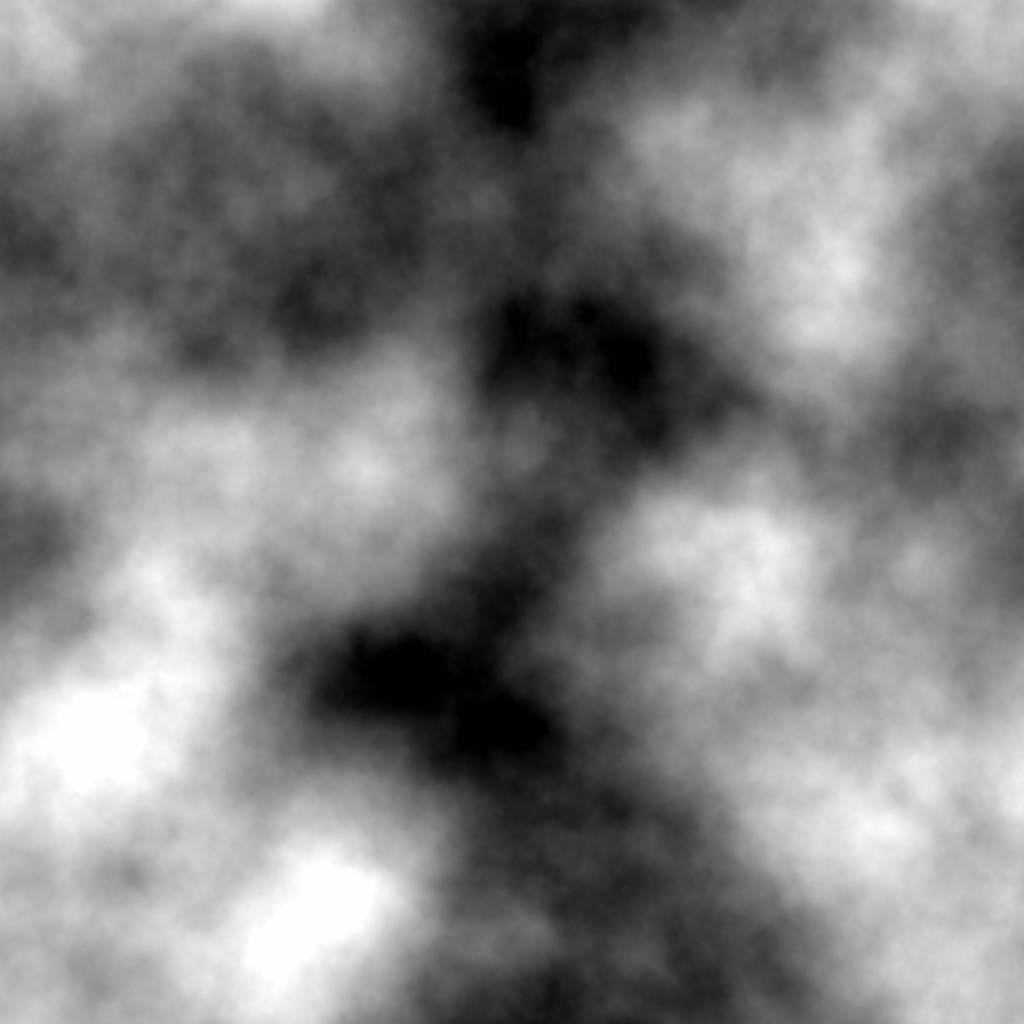
\includegraphics[width=.8\linewidth]{img/brown_noise}
  \caption{Červený, někdy též Brownův šum} 
\end{subfigure}%
\end{tabular} 
\caption{Ukázky různých šumů.} 
\label{obr:noise:example} 
 
\end{figure}
\section{Gabor patch}

Gabor filter (v českých textech někdy označovaný jako Gaborova vlnka) je
lineární filtr používaný ve zpracování obrazu, chceme-li detekovat signál
mající danou frekvenci a směr, který se vyskytuje kolem daného bodu.

\subsection{Definice}

Hodnotu filtru v daném bodě spočítáme jako součin dvou funkcí. První z nich je
vždy sinus či cosinus (někdy uváděné v podobě komplexní exponenciály, pokud
potřebujeme i reálnou, i imaginární složku). Jeho parametry určují, jaké
vlastnosti má mít signál, který chceme detekovat. Druhé funkci říkáme obálka, a
určuje, na jakém okolí daného bodu signál zkoumáme.

Funkce tedy vypadá jako $$g(x,y) =
\sin\left(2\pi\frac{x'}{\lambda}+\phi\right)*\operatorname{obálka}(x',y'),$$
kde vektor $(x',y')^T$ je vektor $(x,y)^T$ otočený o úhel, který svírá osa $x$
se směrem, podél nějž chceme měřit signál (tento úhel budeme značit $\Theta$),
a posunutý do bodu, v němž chceme měřit signál, $\lambda$ je frekvence signálu,
který hledáme, a $\phi$ je fázový posun.

Jako obálka se používá dvojrozměrná Gaussova funkce, raised cosine, nebo prostá
lineární funkce vzdálenosti. 

Gaussovu funkci vyjádříme jako $$ \operatorname{obálka}(x,y) =
\exp\left(\frac{x'^2 + y'^2}{2\rho}\right),$$ kde $\rho$ je směrodatná odchylka
Gaussovy křivky. Její výhodou je, že chování Gabor filtru, jehož obálku tvoří
Gaussova funkce, je nejlépe popsané. Raised cosine vyjádříme jako 
$$
\operatorname{obálka}(x,y)=
\begin{cases}
 \frac{\cos(\pi\sqrt{x'^2+y'^2}/r)+1}2 &\text{pro $\sqrt{x'^2+y'^2}\leq r$,}\\[1ex]
 0 &\text{jinak,}
\end{cases}
$$ kde $r$ je poloměr oblasti, v níž chceme signál detekovat. Výhodou raised
cosine oproti Gaussově funkci je, že ve vzdálenosti alespoň $r$ od středu
filtru jeho hodnota nabývá nuly. Při výpočtech tedy stačí počítat s malou
oblastí kolem středu (kdežto při použití Gaussovy funkce je nutné počítat s
celým obrazem). Výhodou oproti lineární funkci vzdálenosti je, že raised cosine
se pro většinu aplikací chová dostatečně podobně, jako Gaussova funkce.

\subsection{Použití}

Chceme-li detekovat signál ve vizuálním šumu, spočítáme hodnotu $$s=\sum
g(x,y)*n[x,y],$$ kde $n$ je šum a sumu bereme přes všechny body $(x,y)$, v
nichž jsme naměřili hodnoty šumu. Je-li hodnota $s$  blízko nuly, signál v
daném místě není přítomen, nebo je přítomen s jinými parametry. Vysoké hodnoty
značí, že
signál pravděpodobně přítomen je, hluboce záporné značí, že signál je přítomen,
ovšem s fází posunutou $\pi$.

Gabor filter ale můžeme používat i k samotné tvorbě signálu. Chceme-li vytvořit
v nějakém bodě signál, můžeme spočítat Gabor filter, jako bychom chtěli
detekovat signál s právě takovými parametry, jaké má mít tvořený signál, a
potom ho sečíst se šumem. Takto vytvořenému signálu budeme říkat Gabor patch.

\begin{figure}[h!]
\begin{subfigure}{0.25\textwidth}
  \centering
  
\includegraphics[width=.8\linewidth]{img/gabor1}
\end{subfigure}% 
\begin{subfigure}{0.25\textwidth}
  \centering
  
\includegraphics[width=.8\linewidth]{img/gabor2}
\end{subfigure}% 
\begin{subfigure}{0.25\textwidth}
  \centering
  
\includegraphics[width=.8\linewidth]{img/gabor3}
\end{subfigure}% 
\begin{subfigure}{0.25\textwidth}
  \centering
  
\includegraphics[width=.8\linewidth]{img/gabor4}
\end{subfigure}% 

\caption{Ukázky několika Gabor patchů. Všechny gabor patche jsou 100 pixelů
široké i vysoké. Levý patch má $\Theta = 1/4\pi$, ostatní mají $\Theta =
-1/4\pi$, levý má jako obálku Gaussovu funkci, prostřední dva raised cosine,
pravý lineární funkci vzdálenosti, první, druhý a čtvrtý mají frekvenci (v
cyklech na pixel) $0.1$, třetí $0.02$.} 

\label{obr:gabor:example} 
 
\end{figure}

\section{Úvod do teorie detekce signálu}

Teorie detekce signálu řeší problém rozlišení dvou signálů, případně signálu a
šumu. V této práci se budem zabývat problémem, kdy je potřeba rozhodnout, zda
se v dané ploše nachází signál, či ne. Této úloze budeme říkat A/N problem,
nebo pouze A/N.

V kontextu této úlohy můžou po odpovědi pozorovatele nastat čtyři možné situace:

\begin{itemize}
\item {\it Hit} -- Signál byl přítomen a pozorovatel ohlásil, že signál je
přítomen.
\item {\it Miss} -- Signál byl přítomen ale pozorovatel odpověděl, že signál
přítomen není.
\item {\it Correct rejection} -- Signál nebyl přítomen a pozorovatel odpověděl,
že signál není přítomen.
\item {\it False alarm} -- Signál nebyl přítomen, ale pozorovatel ohlásil, že
přítomen je.
\end{itemize} 

 V této úloze se pozorovatel chová tak,
že si zvolí kritérium (někdy též práh odpovědi), které udává, jaká musí být
pravděpodobnost, že signál je přítomen, aby pozorovatel odpověděl kladně.

\def\P#1{\operatorname{P}\left[#1\right]}
\def\E#1{\mathbb{E}\left[#1\right]}
\def\tP#1{\P{\text{#1}}}

Poté pozorovatel provede pozorování, z nějž získá informaci $s$. Poté spočítá
hodnotu rozhodovací proměnné, tedy spočítá, jaká je pravděpodobnost, že je
signál přítomen. Tato pravděpodobnost se z Bayesovy věty spočítá jako 
%\begin{equation}
\begin{multline*}
\tP{Signál je přítomen| Pozorování dalo informaci $s$} = \\ 
=\frac{\tP{Pozorování dalo informaci $s$
| Signál je přítomen}*\tP{Signál je přítomen}}{\tP{Pozorování dalo informaci
$s$}}\\ \end{multline*}
%\end{equation}
Poté porovná tuto rozhodovací proměnnou s kritériem a podle výsledku tohoto
porovnání odpoví.

Odsud je zřejmé, že zvyšováním kritéria zvedáme pravděprodobnost, že nastane
miss, ale snižujeme pravděpodobnost false alarmu.

\section{Entropie}

Entropií (nazývanou též Shannonova entropie, aby nedošlo k záměně s entropií
tak, jak jí chápe termodynamika) náhodné veličiny se v teorii informace rozumí
střední hodnota informace, kterou nám hodnota této veličiny přinese. Například
mějme náhodné veličiny $X$ a $Y$. $X$ nechť nabývá hodnoty 0 s pravděpodobností
$1/2$ a hodnoty 1 s toutéž pravděpodobností. $Y$ nechť nabývá hodnoty 1 s
pravděpodobností 1 a hodnoty 0 s pravděpodobností 0. Je vidět, že pokud se
dozvíme, jaké hodnoty nabývá veličina $X$, získáme více informace, než když
zjistíme, jaké hodnoty nabývá $Y$.
\def\H{\operatorname{H}}

Hodnotu informace, kterou nám přineslo zjištění, že náhodná veličina $A$ nabývá
hodoty $a$, spočítáme jako $$I(A=a)=\log_b\left(\frac1{\P{A=a}}\right).$$ Jako
základ logaritmu $b$ se běžně používá 2 (což budeme dělat i v této práci), $e$
nebo 10. Všimneme si, že toto vyjádření množství informace je konzistentní s
intuitivní představou, že zjištění, že $A$ nabývá nějaké nepravděpodobné
hodnoty, je cennější, než zjištění, že nabývá nějaké pravděpodobné. Odsud tedy
entropii $\H(A)$ lze vyjádřit jako $$\H(A)=\mathbb{E}[I(A)]=\displaystyle\sum_{a
\in \Omega}\P{A=a}\log_2\frac1{\P{A=a}},$$ kde $\Omega = \{a|\P{A=a} > 0\}$.
Všimneme si, že podle tohoto vzorce je entropie veličiny $X$, tak jak byla
nadefinována v předchozím odstavci, rovna jedné, kdežto  entropie veličiny $Y$
je rovna nule. To je konzistentní s jednou vlastností entropie, totiž s tím, že
říká, že pokud označíme $A^n$ řetězec prvků $\Omega$ s pravděpodobnostním
rozdělením náhodné veličiny $A$, a $\operatorname K$ ideální kompresní
algoritmus (tedy funkce z $\Omega^*$ do ${0,1}^*$), pak
$$\operatorname{lim}_{n\rightarrow\infty} \frac{\mathbb{E}[|K(A^n)|]}{n} =
\H(A).$$ Neformálně řečeno nám tedy entropie říká, kolik bitů v průměru
potřebujeme na uložení hodnoty náhodné veličiny $A$.

Podobně jako u pravděpodobnosti můžeme poměrně přímočaře nadefinovat i   
podmíněnou entropii $\H(A| B)$

\section{Modely pozorovatele}

V této práci se budeme zabývat úlohou, kdy pozorovatel hledá gabor patch v
kruhovém poli, v němž se nachází růžový šum. Předchozí výzkum ukázal, že lidští
pozorovatelé v této úloze využívají krátkých pohledů a rychlých pohybů očí.
Jednomu takovému krátkému pohledu budeme říkat {\it fixace}. Oční pohyb mezi
fixacemi nemá v české literatuře zaužívané pojmenování, v anglické se používá
termín {\it saccade}, v této práci mu tedy budeme říkat {\it sakáda}. Pojem
sakáda přirozeně aplikujeme i na simulované (tj. ne liské) pozorovatele, kde ho
budeme chápat jako vektor v $\mathbb{R}^2$ mezi středy dvou po sobě jdoucích
fixací. Jednotlivé fixace trvají přibližně $200$--$300 \operatorname{ms}$.

Abychom ale mohli hodnotit fixace lidského pozorovatele, potřebujeme mít nějaký
model, který nám bude říkat, jak se chová optimální pozorovatel. Nejprve ale
stručnou odbočku:

\subsection{$d'$ mapa}

Ještě předtím, než začneme zjišťovat, podle jakého modelu se chová lidský
pozorovatel, je nutné zjistit, kolik informace člověk jednou fixací získá. Je
například zjevné, že kdyby jedním pohledem bez ohledu na to, kam se dívá,
získal stejné množství informace o všech možných polohách cíle, jsou všechny
modely ekvivalentní. Proto je potřeba najít tzv. $d'$ mapu, funkci, která nám
pro každé dva body $x$, $y$ řekne, jaká je pravděpodobnost, že bychom
zaznamenali cíl na pozici $y$, pokud se podíváme na pozici $x$. U pozadí s
uniformními nebo téměř uniformními lokálními kontrasty lze tuto funkci
zjednodušit, stačí, když budeme pro každý bod $x$ vědět, jakou s jakou
pravděpodobností bychom objevili cíl, kdyby se nacházel v bodě $x$, pokud
zafixujeme střed.

Předchozí výzkum ukázal, že u běžného člověka je $d'$ mapa poměrně
nepravidelná, ale dá se s přijatelnou přesností aproximovat mapou, kde křivky
spojující body se stejnou hodnotou $d'$ jsou tvořeny čtyřmi čtvrtelipsami
(jednou v každém kvadrantu) se středem v počátku. Takovou $d'$, s
excentricitami a velikostí poloos danou hodnotou $d'$ a individuálními
vlastnostmi pozorovatele a cíle. 

Ke kompletnímu vyjádření aproximace funkce $d'$ potřebujeme celkem 6 hodnot,
které závisí na konkrétním pozorovateli a cíli. Jedná se o hodnotu $d'_0 =
d'(0,0)$, hodnot $e_L$, $e_R$, $e_U$ a $e_D$, které určují vzdálenost ve čyřech
základních směrech takovou, že v nich je hodnota $d'$ poloviční oproti počátku,
a hodnotu $\beta$ popisující sklon této funkce. Funkci $d'$ pak vyjádříme jako
$$ d'(x,y) = \frac{d'_0}{1+\left(\frac{x^2}{e_H^2}+\frac{y^2}{e_V^2}
\right)^\beta}, $$ kde $e_H$ je rovno $e_L$ pro záporná $x$ a $e_R$ pro kladná,
a $e_V$ je rovno $e_D$ pro záporná $y$ a $e_N$ pro kladná.


\subsection{Modely chování pozorovatele}

Všechny modely, které zde budeme zkoumat, vypadají tak, že mají tzv. {\it Mapu
posteriorních pravděpododbností}. V této mapě je pro každou lokaci, kde by
signál (též cíl) mohl být, uvedeno, jaká je pravděpodobnost, že se na ní cíl
nachází vzhledem k informaci, kterou již o dané lokaci pozorovatel získal. Ve
chvíli, kdy na nějaké lokaci pravděpodobnost přesáhne kritérium, pozorovatel
ukončí hledání a ohlásí nalezení cíle na této lokaci.

V rámci předchozího výzkumu bylo otestováno mnoho modelů, jako například
pozorovatel, který volí fixace náhodně nebo pozorovatel, který volí fixace co
nejdále od míst, která již zafixoval. Všechny tyto modely se ale ukázaly jako
nevhodné, vzhledem k tomu, že v praxi dosahují mnohem horších výsledků (měřeno
pomocí střední hodnoty počtu fixací před nalezením cíle) než lidský
pozorovatel.

\subsubsection{MAP pozorovatel}

Nejjednoduší model, který dosahuje podobných výsledků, jako lidský pozorovatel,
je tzv. MAP\footnote{Z anglického \uv{Maximum Aposteriori Probability}.}
pozorovatel, který vždy zafixuje lokaci, která má v jeho mapě posteriorních
pravděpodobností nejvyšší hodnotu. Tento pozorovatel již dosahuje podobných
výsledků jako lidský, ale jeho strategie fixací neodpovídá strategii, jakou
volí lidský pozorovatel. Lidský pozorovatel umístí svoji první fxaci do středu
scény. Ostatní fixace jsou pak rozmístěny v okolí kružnice se středem ve středu
scény a poloměrem rovným přibližně $2/3$ poloměru scény, s preferencí pro horní
a spodní okraj. MAP pozorovatel oproti tomu vybírá každou lokaci se zhruba
stejnou pravděpodobností.

\subsubsection{Ideální Bayesovský pozorovatel}

Ještě o malinko lepších a hlavě statisticky lidskému pozorovateli bližších
výsledků bosahuje model Ideálního Bayesovského pozorovatele.  

Ideální Bayesovský pozorovatel (dále IBO) je pozorovatel, který $T+1$ lokaci
vybírá tak, aby maximalizoval pravděpodobnost, že v následujícím kroku odhalí
cíl. Vybere tedy lokaci 
\begin{equation}\label{IBOnext}k_{opt}(T+1) = \displaystyle{\operatorname{arg\ 
max}}_{k(T+1)} \left(\displaystyle\sum_{i\in L} p_T(i)\P{p_{T+1}(i)\geq c|i,
k(T+1)}\right),
\end{equation} 
kde $p_N$ je mapa posteriorních pravděpodobností po $N$-té
fixaci, $L$ je množina všech potenciálních lokací cíle a $c$ je kritérium,
které musí hodnota v mapě posteriorních pravděpodobností překročit, aby bylo
ukončeno hledání a nahlášeno nalezení cíle. Výraz $\P{p_{T+1}(i)\geq c |
i,k(T+1)}$ pak tedy znamená \uv{pravděpodobnost, že po $T+1$ fixaci bude
ukončeno hledání a nahlášen signál v lokaci $i$, za podmínky, že tam signál
opravdu je a byl zafixován bod $k(T+1)$}. 

IBO však ale též není příliš pravděpodobný  kandidát na model, podle nějž se
lidé chovají.  Ač má jeho vyhledávání podobné statistické vlastnosti, jako
vyhledávání lidského pozorovatele, můžeme si všimnout, že přinejmenším
přímočaré vyhodnocení výrazu \eqref{IBOnext} je kubické v počtu potenciálních
lokací (výpočet druhého činitele součinu v sumě je lineární, suma sama je přes
lineárně mnoho členů, a vnější maximum má též lineárně mnoho možných voleb
$k(T+1)$). Lidský pozorovatel při vyhledávání volí další fixaci přibližně
třikrát až čtyřikrát za vteřinu, je tedy nepravděpodobné, že by lidský mozek
dokázal takový výpočet provést. 

\subsubsection{ELM pozorovatel}

ELM\footnote{z anglického \uv{Entropy limit minimization}.} pozorovatel je
pozorovatel, který při výběru následující fixace minimalizuje střední hodnotu
entropie náhodné veličiny určující lokaci cíle. Tu spočítáme jako
\begin{equation}\label{EntropyBasic}\E{\H(T+1)|k(T+1)}=-\E{\displaystyle\sum_{i\in
L}p_{T+1}(i)\log_2p_{T+1}(i)|k(T+1)}.\end{equation} V ZDROJ09 se však zjistilo,
že vyjádření hodnoty entropie podle vzorce \eqref{EntropyBasic} je sice
netriviální, ale lze ho dobře aproximovat případem, kdy pošleme v limitě $|L|$
do nekonečna. Pak dostáváme výraz $$ \E{\H(T+1)|k(T+1)}= \H(T) -
\displaystyle\sum_{i\in L} p_T(i)d'^2(i-k(T+1)),$$ kde v posledním členu bereme
lokace jako vektory od počátku k nim. Člen $\H(T)$ navíc nezávisí $k(T+1)$,
takže s ním vůbec nemusíme počítat a k minimalizaci entropie nám stačí
maximalizovat hodnotu sumy. 

